\chapter{Diseño del layout de un canal de lectura}

El diseño del layout de un canal de lectura en el contexto de un proyecto suele
ser una tarea que ocupa gran parte del periodo de diseño, y además es recomendable
abordar en las primeras fases del proyecto, ya que como hemos comentado, el
layout va a influir, en mayor medida que otros bloques, en el diseño del mismo.
Por tanto, el diseño del canal de lectura suele ser un proceso iterativo:
diseñodel esquemático, layout, extracción, simulación y eventual rediseño.\\

\section{Jerarquización}

A la hora de estructurar el diseño de layout de cualquier bloque repetitivo, como
es el canal de lectura, es básico idear una estrategia en cuanto a la jerarquización
del mismo, ya que usualmente no se trata de un simple array de instancias iguales
situadas una al lado de la otra.\\

Por otra parte, existen estructuras que pueden requerir diferentes periodicidades.
Y también hay que adaptarse a la resolución del array, en este caso, al número de
columnas. Como ya hemos visto a lo largo de la descripción del esqumático del canal
nuestra unidad básica de un canal de lectura, a la que nos referiremos como
$ro\_chx1$, ocupará una anchura de 2 columnas de píxeles, es decir, una anchura
de $10\mum$. En esa anchura tiene que ser posible incluir todos los bloques que
se repiten por canal, es decir, la fuente de corriente y el ADC de una columna de
píxeles.\\

En un siguiente nivel de jerarquía, incluiremos 8 canales unitarios y sus
correspondientes bloques de polarización (PXCS\_BIAS y ADC\_BIAS), que como vimos,
están compartidos por cada 8 canales. De esta forma, el bloque $ro\_chx8$
tendría una anchura de $10\mum \times 8 = 80\mum$, y tendríamos canales para
leer 16 columnas de píxeles.\\

Desde 16 columnas hasta las columnas totales del array podemos elegir varios niveles
de jerarquías intermedios. Considerando que nuestro array tiene la estructura
mostrada en el capítulo \ref{cap:pxa_array}, en la figura \ref{fig:pxa_array},
con 2560 columnas activas y 64 columnas oscuras, vamos a hacer una jerarquía que
cubra esos 64 píxeles, es decir, 32 canales, por lo que se llamará $ro\_chx32$ e
instanciará 4 unidades de $ro\_chx8$.\\

Para completar las 2560 columnas de píxeles activos, solo hay que instanciar 40
de los bloques de 32 canales. Y para completar el array, tan solo hay que añadir
2 canales (4 píxeles) a izquierda y derecha de la zona activa (píxeles dummy), y
un bloque de 32 canales en la zona de las columnas oscuras, con sendos pares de
canales a izquierda y derecha para hacer las columnas oscuras dummy.\\

\subsection{Redundancia}

En todo diseño microelectrónico, debido a defectos en la fabricación, ciertos
dispositivos pueden resultar completamente inutilizables o, al menos, con prestaciones
por debajo de lo esperado en relación al resto de dispositivos equivalentes.
Esto se acentua en casos como un canal de lectura, en los cuales la integración
y la congestión de rutado y dispositivos es muy alta, y además tiene un patrón
altamente simétrico y periódico.\\

Con el paso del tiempo, los fabricantes de sensores de imagen han detectado que
el canal de lectura sufre de considerablemente más fallos que el resto de circuitos
en el sensor, y por consiguiente es uno de los principales contribuyentes a la
disminución del ``\textit{yield}'' (del inglés: rendimiento), que da cuenta del
porcentaje de sensores por oblea que no funcionan o son defectuosos, lo que va
en contra del beneficio económico.\\

Para tratar de disminuir este problema, se suele poner en práctica el uso de canales
redundantes, esto es, canales adicionales que podrían ser usados en el caso de que,
una vez fabricado el chip, se detecten fallos en un canal concreto.\\

Para esto se añade un canal adicional cada cierto número de canales y mediante un
sistema de llaves a la entrada de todos los canales podemos redireccionar la
salida todos los píxeles en el rango afectado y posteriores al canal del fallo,
hacia el siguiente canal. Con esto se puede ver fácilmente que podemos solucionar
tantos fallos como canales redundantes sean incluidos, siempre y cuando no se
produzca más de un fallo por región.\\

\begin{figure}[h]
	\includesvg[width=\textwidth]{svg/redundancy.svg}
	\caption{Ejemplo del funcionamiento del sistema de redundancia}
	\label{fig:redundancy}
\end{figure}

En la figura \ref{fig:redundancy} vemos un ejemplo de aplicación del sistema de
redundancia donde tendríamos un canal redundante por cada 4. En el que caso de que
fallen los canales 2 y 5 mostrados en la imagen, el bloque de redundancia colocado
en la parte superior del canal de lectura podría dirigir cada columna a la siguiente,
de la forma que muestran las líneas rojas.\\

Como ya se puede intuir, la anchura del canal de lectura, en el supuesto de usar
redundancia se tiene que ver reducida con objeto de incluir un canal adicional
cada cierto tiempo. En nuestro caso vamos a incluir un canal redundante por cada
grupo de 32 canales funcionando. Con esto, haciendo una sencilla cuenta, podemos
establecer la nueva anchura en $9\mum$ en vez de las $10\mum$ originales. Esto nos
permite además tener una anchura sobrante cada 33 canales que será:
$32\cdot 10\mum - 33\cdot 9\mum = 23\mum$ de anchura sobrante. Este espacio lo
podemos usar para por ejemplo subir las tensiones de polarización desde los BIAS
a las líneas horizontales en los correspondientes bloques.\\

\section{Estructura de layout de una columna del canal}

La estructura completa se muestra al final de capítulo (\ref{fig:ro_chx1}) en un diagrama
simplificado del layout de una columna de canal ($ro\_chx1$), mostrando los bloques más
importantes, sus tamaños y sus conexiones.

Una vez establecida una jerarquía clara, y suponiendo el uso de la redundancia ya
tenemos establecida una anchura para el layout de una columna de nuestro canal.
En esta anchura deberemos incluir todos los bloques descritos en el esquemático
tratando de hacerlo lo más compacto posible para ahorrar área en la dirección vertical.\\

Como hemos introducido en el apartado anterior, el bloque de redundancia será
el primero que nos encontraremos por la parte superior, más cerca del array de
píxeles. Para esto además tiene que existir un rutado que transforme las salidas
de los píxeles, espaciadas cada $5\mum$ a las entradas de los bloques de redundancia,
espaciadas 2 cada $9\mum$.\\

Lo siguiente que tenemos es la fuente de corriente, que es una por cada columna
de píxeles, es decir, dos en cada canal unitario, y se van a colocar una encima
de otra ocupando ambas la anchura del canal, $9\mum$.\\

Inmediatamente debajo colocaremos el bloque de polarización de las fuentes de
corriente, PXCS\_BIAS, que como se comparte para 8 canales, en la unidad $ro\_chx1$,
dejaremos un hueco de la altura necesaria, que se establecerá en función de la altura
del BIAS.\\

Por debajo del PXCS\_BIAS, vamos a colocar los ADC, que tiene que haber dos por
cada columna de píxeles si queremos usar la técnica de ping-pong. En nuestro caso
esto significa tener que implementar 4 ADCs idénticos dispuestos en vertical ocupando
las $9\mum$ de anchura del canal.\\

Por último, bajo los 4 convertidores iría el Bias del ADC, que tambíen se comparte
por cada 8 canales, por lo que tampoco estaría incluida en columna unitaria.\\

\section{Problemas de layout que afectan al diseño del canal de lectura}

\subsection{Consumo}

El consumo de un bloque tan grande como es el canal de lectura siempre es algo a
tener muy en cuenta a la hora de modelar las alimentaciones que debe tener y
cómo afectan estas al funcionamiento del propio bloque y del resto del sensor.\\

En muchas ocasiones no es tan importante que un bloque tenga un consumo alto,
como la dinámica con la que se produzca ese consumo. Si un bloque tiene un alto
consumo, pero lo hace de manera más contínua que otro que tiene grandes picos de
alto, quizás afecte menos al rendimiento total del circuito. En el caso del
canal de lectura esto es muy importante porque muchos de los procesos se producen
de forma simultánea en todos los canales a la vez. Por esta razón hay que tener
especial cuidado a cómo se programan los tiempos de lectura y comparación,
y, lo más importante, realizar exhaustivas simulaciones usando extraído de parásitos
y modelando muy bien las alimentaciones y los acoplos que podemos tener. Este tema
se tratará en más detalle en el apartado \ref{cap:simulacion} sobre simulaciones.\\

Otro punto importante a considerar es que el canal de lectura va a ser alimentado,
tan solo por ambos extremos. Esto va a generar una curvatura en las alimentaciones
que puede traer problemas, manifestándose como un gradiente en la imagen final.
Las tensiones de polarización del los bloques de bias, están generadas localmente
y referidas a una tierra con curvatura por lo que unos ADC y otros
podrían tener tener diferente tiempo de conversión, por ejemplo.\\

\begin{figure}[ht]
	\includesvg[width=\textwidth]{svg/adc_poly_short.svg}
	\caption[Consecuencias de la curvatura en la alimentación del canal]
	{Curvatura en la tensión de tierra y una tensión de polarización a lo largo del canal,
	donde se diferencian 3 posibles estrategias a la hora de cortocircuitar las
	tensiones de polarización.}
	\label{fig:adc_poly_short}
\end{figure}

Para tratar de corregir este efecto, se suelen cortocircuitar las tensiones de polarización
entre todos los canales del array. En la imagen \ref{fig:adc_poly_short} podemos ver
3 casos. El caso (a) lo que ocurriría si no cortocircuitamos los adc\_bias,
el caso (b), si lo hacemos con una línea metálica, con baja resistividad,
y el caso (c) si lo hacemos con una línea más resistiva, de poly.
La solución elegida es la última porque suaviza mucho mejor los voltajes de polarización
entre los diferentes canales, al adaptarse a la irremediable curvatura de la tierra.\\

\subsection{Acoplos}

Otro tema crítico en el diseño del layout del canal de lectura es los posibles acoplos
entre señales debidos principalmente a la apilación de canales requerida por la
paralelización de varios píxeles y por el uso de la técnica de ping-pong. Es más,
el uso del ping-pong hace incluso más crítico este tema, ya que va a significar
que en los mismos periodos de tiempo van a concurrir fases de muestreo y comparación
en canales que se encuentran apilados.\\

Algunas líneas como el $adc\_take$ que saldría de un canal superior, va a tener que,
obligatoriamente, pasar por encima de algún canal inferior que esté haciendo
\textit{sampling}. Y, debido a que la transición del \textit{take}, se produce
en un momento indeterminado, en función de la luz captada por el píxel leído, puede
coincidir que dicha transición se produzca en el periodo final de una fase de
muestreo del otro canal. Si esta señal tiene un acoplo con uno de los nodos de
entrada del comparador, o con los condensadores, puede ocurrir que se produzca
un pico en la señal que se está muestreando y al ser el final del periodo de muestreo,
no dar tiempo a que se reestablezca y haber finalmente modificado el valor leído.\\

\subsection{Condensadores del ADC}

Los dos condensadores que debe haber por cada ADC son otro punto a tener en
consideración, ya que son una parte fundamental del mismo. Lo primero que
hay que decir es que suelen ser grandes, más aún si se trata de un sensor de
bajo ruido, esto es, que está destinado a captar imágenes con escasa iluminación
y se requieren altos rango dinámico y resolución, por lo que se necesitan condensadores
mayores.\\

También son grandes porque habitualmente se implementan usando condensadores
metálicos, que usan placas de metal 3 y 4 una sobre la otra. Este tipo de condensador
tiene una densidad de capacidad por unidad de área menor que otros como los tipo
MOS descritos en \ref{cap:condensadores}, pero se usan por la mayor linealidad que
estos últimos.\\

Un punto a tener atención es al apantallado de estos condensadores entre los de
las columnas vecinas. Si entre ellos hubiera una capacidad alta, podría haber
una transferencia de carga si el valor almacenado en uno de ellos es muy diferente
al otro, lo que crearía un efecto de desenfoque de los bordes abruptos en la imagen.\\

Otro problema que introducen los condensadores, en concreto, que estén fabricados
los metales superiores 3 y 4, es que las señales que se distribuyen verticalmente,
como el $adc\_take$ y la salida del píxel, que habitualmente se rutan en los metales
más altos para facilitar el apantallado, van a tener que bajar para pasar por debajo
de los condensadores. Esto va a posibilitar que se acoplen a otras señales que se ruten
en metales inferiores.\\

\subsection{Distribución de señales horizontalmente}

Como ya se ha comentado en otros apartados, la distribución horizontal de las
señales de control, o \textit{fases}, necesita especial atención, sobre todo
si el array consta de muchas columnas.\\

Una de las principales señales horizontales es la rampa analógica. En el caso de
producirse un retraso en la propagación de esta, los valores leídos serían mayores
de los verdaderos. Por lo tanto siempre trataremos de disminuir dicho tiempo de
propagación, lo que se consigue con baja resistencia, esto es, mayor anchura de
líneas, y menor capacidad, mayor espaciado con otras líneas o con el substrato.
Por otra parte, es bueno que no se ensucie con posibles acoplos con señales verticales,
por lo que habitualmente se elige rutar la rampa en metal Top de $10\mum$ de anchura,
sobre una capa de Metal 3 conectado a tierra como apantallamiento.\\

Siempre y cuando el error producido por el retraso de la rampa quede por debajo
de un LSB, no se vería nada en la imagen debido a este retraso. Si no es así, y es
inevitable un pequeño retraso, siempre se puede corregir posteriormente, ya que
se trata de un error de patrón fijo \textit{``Fixed Pattern Noise''} o FPN, que
en la fase de caracterización del sensor, se podría corregir mediante unos
parámetros de ajuste por canal.\\

En cuanto a los retrasos en las fases, debido a que estos afectan a las señales de
muestreo, debemos tener más cuidado puesto que podría darse el caso extremo de
que las fases de muestreo se descuadren demasiado con la señal de \textit{sel} del
píxel y que perdamos periodo de muestreo efectivo. Esto se debe corregir tratando
de ecualizar la constante de tiempo la señal de \textit{sel} con el resto de
fases. Hay que recordar que normalmente la primera tiene mucha menos libertad a la
hora del diseño. La anchura y la capacidad del \textit{sel} está muy acotada
por el complejo diseño del layout del píxel. Por lo tanto solo podemos actuar
sobre el diseño de las líneas de las fases del canal. Debemos comprobar bien
anchuras, acoplos a otras líneas y tamaño y cantidad de dispositivos que cuelgan
de ellas, tratando de equilibrar las constantes de tiempo de todas ellas.\\

Para esto, una vez más, es muy importante una cuidada extracción de parásitos y
exhaustivas simulaciones post-layout, en diferentes canales a lo largo de todo el
array.\\

\begin{figure}[h]
\centering
\begin{minipage}{0.48\textwidth}
	\includesvg[width=\textwidth]{svg/ro_chx1_layout.svg}
	\caption[Floorplan de una columna de canal de lectura]
	{Floorplan del layout de una columna del canal de lectura ($ro\_chx1$),
	donde se puede ver la disposición de los bloques principales y sus conexiones
	más importantes}
	\label{fig:ro_chx1}
\end{minipage}
\hfill
\begin{minipage}{0.48\textwidth}
	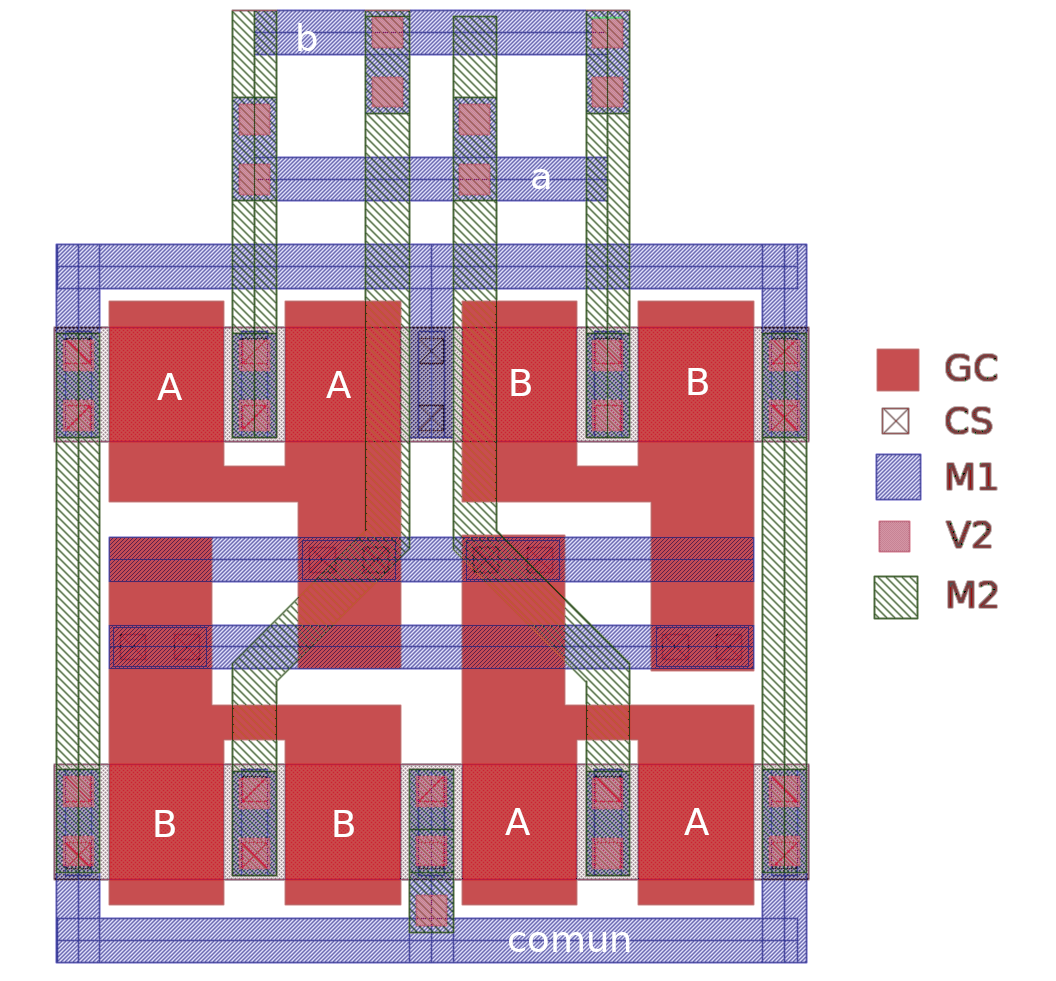
\includegraphics[width=\textwidth]{img/OTA_simple_layout.png}
	\caption[Layout del par diferencial del OTA del comparador]
	{Layout del par diferencial del OTA del comparador, donde se ve
	la estructura de centroide común usada para minimizar el mismatch.
	A y B son los dos transistores del par diferencial $M_1$ y $M_2$ y ``comun'' es
	el nodo que viene de la fuente de corriente $M_5$ del OTA. Véase
	esquemático en \ref{fig:ota_sch}}
	\label{fig:ota_simple_layout}
\end{minipage}
\end{figure}
